\documentclass[]{beamer}
%\documentclass{article}
%\usepackage{beamerarticle}

\mode<presentation>
{
  \usetheme{Warsaw}
  % or ...

  \setbeamercovered{transparent}
  % or whatever (possibly just delete it)
}


\usepackage[english]{babel}
% or whatever

\usepackage[utf8]{inputenc}
% or whatever

\usepackage{times}
\usepackage[T1]{fontenc}
\usepackage{tikz}
\usetikzlibrary{arrows.meta}

%%%%%%%%%%%%%%%%%%%%%%%%%%%%%%%%%%
%%                         PACKAGES                      %%
%%%%%%%%%%%%%%%%%%%%%%%%%%%%%%%%%%
\usepackage{hyperref,ctable}
\usepackage{graphicx}
\usepackage{tikz}                    % For flowchart
\usetikzlibrary{shapes,arrows} % For flowchart


%%%%%%%%%%%%%%%%%%%%%%%%%%%%%%%%%%
%%                           COLORS                        %%
%%%%%%%%%%%%%%%%%%%%%%%%%%%%%%%%%%
%AU COLORS
\definecolor{aublue}{RGB}{25,33,129}
\definecolor{aured}{RGB}{244,28,31}

%Red
%\setbeamercolor{titlelike}{bg=aured,fg=white}
\setbeamercolor{structure}{bg=black!25!aured, fg=aured}
%\setbeamercolor*{palette primary}{fg=white,bg=aured}
%\setbeamercolor*{palette quaternary}{fg=white,bg=aublue}

%Blue
\setbeamercolor{titlelike}{bg=aublue,fg=white}
%\setbeamercolor{structure}{bg=black!25!aublue, fg=aublue}
\setbeamercolor*{palette primary}{fg=white,bg=aublue}
\setbeamercolor*{palette quaternary}{fg=white,bg=black!75!aublue}

\setbeamercolor{local structure}{fg=aured,bg=gray!60!aured}
\setbeamercolor{alerted text}{fg=aured}

\newenvironment{concept}[1]%
	{
	\setbeamercolor{background canvas}{bg=aured!10!white}%
	\setbeamercolor{frametitle}{bg=aured}%
	\setbeamercolor{frametitle right}{bg=aured}
	\setbeamercolor{alerted text}{fg=aured}%
	\begin{frame}{Concept}%
	\alert{\bfseries \large #1\\[2em]}}{%
	\end{frame}%
	}


%%%%%%%%%%%%%%%%%%%%%%%%%%%%%%%%%%
%%                         GRAPHICS                       %%
%%%%%%%%%%%%%%%%%%%%%%%%%%%%%%%%%%
%\graphicspath{{/Users/bader/work/Presentations/Images/}}}}


%%%%%%%%%%%%%%%%%%%%%%%%%%%%%%%%%%
%%                        COMMANDS                       %%
%%%%%%%%%%%%%%%%%%%%%%%%%%%%%%%%%%
\newcommand{\strong}[1]{\textbf{#1}}
\AtBeginSection[]{
  \begin{frame}
  \vfill
  \centering
  \begin{beamercolorbox}[sep=8pt,center,shadow=true,rounded=true]{title}
    \usebeamerfont{title}\insertsectionhead\par%
  \end{beamercolorbox}
  \vfill
  \end{frame}
}



%%%%%%%%%%%%%%%%%%%%%%%%%%%%%%%%%%
%%                     PRESENTATION                   %%
%%%%%%%%%%%%%%%%%%%%%%%%%%%%%%%%%%
\title{Writing Good Questions}

\author[Bader--SOCY 625]
{Michael D.~M.~Bader}

\institute 
{
  Practicum in Sociological Research (SOCY 625)
}
% - Use the \inst command only if there are several affiliations.
% - Keep it simple, no one is interested in your street address.

\date % (optional)
{Week 7}

\subject{Practicum in Sociological Research Slides}
% This is only inserted into the PDF information catalog. Can be left
% out.

% If you have a file called "university-logo-filename.xxx", where xxx
% is a graphic format that can be processed by latex or pdflatex,
% resp., then you can add a logo as follows:

%\logo{\includegraphics[height=1cm]{../../Images/au_logo_50by51px}}
%\logo{\includegraphics[height=1cm]{../../Images/au_logoname_300}}
\logo{\includegraphics[height=1cm]{/Users/bader/work/Presentations/Images/au_logoname_300}}

\subject{Intro to Survey Methods}
% This is only inserted into the PDF information catalog. Can be left
% out. 



% If you have a file called "university-logo-filename.xxx", where xxx
% is a graphic format that can be processed by latex or pdflatex,
% resp., then you can add a logo as follows:

% \pgfdeclareimage[height=0.5cm]{university-logo}{university-logo-filename}
% \logo{\pgfuseimage{university-logo}}



% Delete this, if you do not want the table of contents to pop up at
% the beginning of each subsection:
%\AtBeginSubsection[]
%{
%  \begin{frame}<beamer>{Outline}
%    \tableofcontents[currentsection,currentsubsection]
%  \end{frame}
%}


% If you wish to uncover everything in a step-wise fashion, uncomment
% the following command: 

%\beamerdefaultoverlayspecification{<+->}


\begin{document}

\begin{frame}
  \titlepage
\end{frame}

\section{Using Surveys to Answer Research Questions}

\begin{frame}
\begin{itemize}
\item Research Question
\item Construct
\end{itemize}
\end{frame}


\begin{frame}
\[Y \longleftarrow X\]
\end{frame}

\begin{frame}
\begin{figure}[h!]
\begin{center}
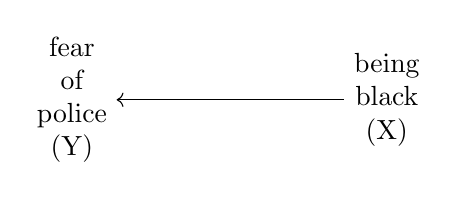
\begin{tikzpicture}
\node (Y) [align=center] at (-2,0) {fear\\ of\\ police\\(Y)};
\node (X) [align=center] at (2,0) {being\\ black\\(X)};
\draw [<-] (Y) to (X);
\end{tikzpicture}
\end{center}
\end{figure}
\end{frame}

\begin{frame}
\begin{center}
\begin{figure}[h!]
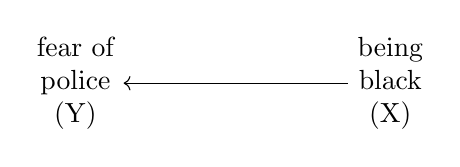
\begin{tikzpicture}
\node (Y) [align=center] at (-2,0) {fear of\\ police\\(Y)};
\node (X) [align=center] at (2,0) {being\\ black\\(X)};
\draw [<-] (Y) to (X);
\end{tikzpicture}
\end{figure}
Being black leads to more fear of the police
\end{center}
\end{frame}

\begin{frame}
\begin{center}
\begin{figure}[h!]
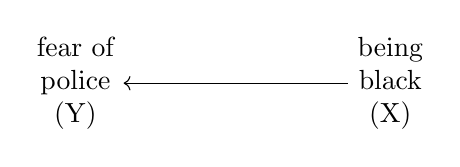
\begin{tikzpicture}
\node (Y) [align=center] at (-2,0) {fear of\\ police\\(Y)};
\node (X) [align=center] at (2,0) {being\\ black\\(X)};
\draw [<-] (Y) to (X);
\end{tikzpicture}
\end{figure}
\alert{Being black} leads to more \alert{fear of the police}
\end{center}
\end{frame}

\begin{frame}
We need \textbf{two} valid constructs:
\begin{enumerate}
\item Race
\item Fear of Police
\end{enumerate}
\end{frame}

\begin{frame}
\begin{center}
\includegraphics[scale=1]{../../Week2-InferenceAndError/images/GrovesCh2Fig2Measurement.pdf}
\end{center}
\end{frame}

\begin{frame}
\begin{enumerate}
\item What is race? \pause
\item How do we measure race with survey question(s)? \pause
\item How will people respond to the question? \pause
\item How will we edit the response? 
\end{enumerate}
\end{frame}


\begin{frame}
\begin{enumerate}
\item What is ``fear of the police''? \pause
\item How do we measure ``fear of the police'' with survey question(s)? \pause
\item How will people respond to the question(s)? \pause
\item How will we edit the response? 
\end{enumerate}
\end{frame}

\begin{frame}
Now we need to measure the relationship: 
\[Y_i = \beta_0 + \beta_1 X_i + \epsilon_i \]
\end{frame}


\section{Testing to Write Good Questions}


\begin{frame}
Groves, et al.\ (2009) lay out three standards for good questions: 
\begin{enumerate}
\item Content
\item Cognitive
\item Usability 
\end{enumerate}
\end{frame}

\begin{frame}
\begin{itemize}
\item Expert reviews
\item Focus group discussions
\item Cognitive interviews
\item Field pretests
\item Spit ballot or randomized experiments
\end{itemize}
\end{frame}

\begin{frame}
Groves, et al.\ (2009)\\
``The `content standard' for questions is whether or not they are asking for the right information.''
\begin{enumerate}
\item From the point of view of analysis
\item Whether respondent can provide the info
\end{enumerate}
\end{frame}

\begin{concept}{reliability}
how likely is it that you will get the same (or consistent) responses when measuring the same construct? 
\end{concept}

\begin{frame}
Response variance (opposite of reliability)
\[\frac{1}{2N}\sum_i\left(Y_{i1}-Y_{i2}\right)^2\]
\end{frame}

\begin{frame}
Multiple indicators 
\[ \alpha = \frac{k\overline{r}}{1+(k-1)\overline{r}} \]
\end{frame}


\end{document}


